\chapter{Introduction}
\label{chap:introduction}

\section{Motivation and the research needs}
Boolean satisfiability (SAT)~\cite{SATHandbook} has been successfully applied to numerous research fields
including artificial intelligence~\cite{Nilsson2014,Russell2020},
electronic design automation~\cite{Marques2000,Wang2009},
software verification~\cite{Jhala2009, Berard2013}, etc.
The tremendous benefits have encouraged the development of more advanced decision procedures
for satisfiability with respect to more complex logics beyond pure propositional.
For example,
solvers for majority SAT (MAJSAT) decide whether the majority of the assignments satisfy a propositional formula,
and its functional problem is known as model counting~\cite{SATHandbook-ModelCounting};
quantified Boolean formula (QBF)~\cite{Narizzano2006,SATHandbook-QBF} allows both existential and universal quantifiers;
stochastic Boolean satisfiability (SSAT)~\cite{Littman2001,SATHandbook-SSAT} models uncertainty with randomized quantification;
dependency QBF (DQBF)~\cite{Balabanov2014,Scholl2018} equips Henkin quantifiers to describe multi-player games with partial information;
and solvers of the satisfiability modulo theories (SMT)~\cite{Moura2011,HBMC-SMT} accommodate first order logic fragments.
Due to their simplicity and generality,
various satisfiability formulations are under active investigation.

Among various generalizations of Boolean satisfiability,
\textit{stochastic Boolean satisfiability} (SSAT)~\cite{SATHandbook-SSAT} is a logical formalism
for problems endowed with randomness.
First formulated by Papadimitriou,
SSAT is interpreted as \textit{games against nature}~\cite{Papadimitriou1985}.
Nondeterministic factors are introduced into the world of propositional logic
through the creation of the \textit{randomized quantifier}.
A Boolean variable $x$ can be randomly quantified with a probability $p\in[0,1]$ in an SSAT formula
by a randomized quantifier $\random{p}$ that requires $x$ to take the Boolean value
\true with probability $p$ and
\false with probability $1-p$.
Via randomized quantifiers,
a variety of computational problems inherent with uncertainty can be encoded into SSAT formulas,
such as propositional probabilistic planning~\cite{Littman1998},
Bayesian-network inference~\cite{Cooper1990,Jensen1996,Bacchus2003},
and the analysis of partially observable Markov decision process (POMDP)~\cite{Majercik2003}.

While SSAT has been employed to solve various AI problems,
to the best of our knowledge,
it has not yet been applied to analyze VLSI systems,
and how VLSI systems would benefit from the probabilistic reasoning of SSAT remains unclear.
Conventionally, uncertain system behavior is undesirable and
would be mitigated by employing techniques such as
error detection~\cite{Constantinescu2003} and error correction~\cite{Mitra2006}.
Nevertheless, in the post-Moore's era,
the variability and uncertainty of manufacturing at the atomic level
make devices under miniaturization sensitive to process variation and environmental fluctuation.
As a result, the manufactured ICs may exhibit uncertain probabilistic behavior,
which imposes serious challenges to the design of reliable systems.

Recent research efforts have been made to accept the inevitable imperfection of devices
based on the notions of \textit{approximate design} and \textit{probabilistic design}.
In both notions, a system's behavior may deviate from its expected specification;
however, this deviation is deterministic in the former case but probabilistic in the latter case.
Despite the advancements made by prior endeavors,
the analysis and synthesis of probabilistic design have gained relatively less attention.
Hence,
\textbf{there is a research need of a framework to evaluate probabilistic design},
and SSAT stands up as a suitable logical formalism to address the need.
(In the following,
the term ``design'' is used as a general term to refer to a single design instance,
a set of design instances,
or design process;
the term ``synthesis" is referred to as the design automation process
transforming a system under design from high-level system specification to low-level circuit implementation.)

SSAT is closely related to two generalizations of Boolean satisfiability:
\textit{model counting} of propositional formulas and \textit{quantified Boolean formulas} (QBFs).
Given a propositional formula, model counting asks to compute the number of its satisfying assignments.
In the weighted version, weights are assigned to the Boolean variables in the formula,
and the goal is to compute the summation of weights of the satisfying assignments.
Algorithms for model counting are under active development in recent years.
In addition to \textit{exact} model counting~\cite{Sang2004,Sang2005ModelCounting},
\textit{approximate} model counting~\cite{Gomes2006,Gomes2007,Chakraborty2016}
has been investigated to improve scalability by relaxing exactness.
On the other hand, from the perspective of the computational complexity,
solving an SSAT formula lies in the PSPACE-complete~\cite{Stockmeyer1973} complexity class,
the same as solving a QBF.
Many endeavors have been invested in the algorithmic improvement~\cite{SATHandbook-QBF}
and solver evaluation~\cite{Narizzano2006} for QBF.

Nevertheless, in spite of its broad applications and profound theoretical values,
SSAT has drawn relatively little attention compared to SAT, model counting, or QBF.
Most prior efforts for SSAT solving are based on the conventional
Davis-Putnam-Logemann-Loveland (DPLL) search~\cite{Davis1962},
which suffers from the scalability issue when problem sizes grow.
Therefore, \textbf{there is a research need to develop novel algorithms to enhance the scalability of SSAT solving},
and the recent advancements of SAT/QBF solving and model counting can be leveraged to help the algorithm design.

In spite of its rich expressiveness to encode problems ranging from AI to VLSI,
SSAT is limited by its descriptive power within the PSPACE complexity class.
More complex problems with nondeterminism might not be succinctly modeled as SSAT formulas.
As a result, \textbf{there is a research need of a logical formalism for problems beyond PSPACE and with uncertainty.}

Finally, most research work regarding SSAT solving was done
before the year 2010~\cite{Majercik1998,Majercik2003,Majercik2004,Majercik2005,Teige2010,SATHandbook-SSAT}.
Open-source implementations and SSAT instances for testing are barely available,
which hinder the understanding of the algorithmic details and empirical solver comparison.
Consequently, \textbf{there is a need to provide open-source implementations and databases of SSAT instances to facilitate convenient evaluation of different algorithms and drive further advancements.}

\section{Our contributions}
\begin{figure}[t]
      \centering
      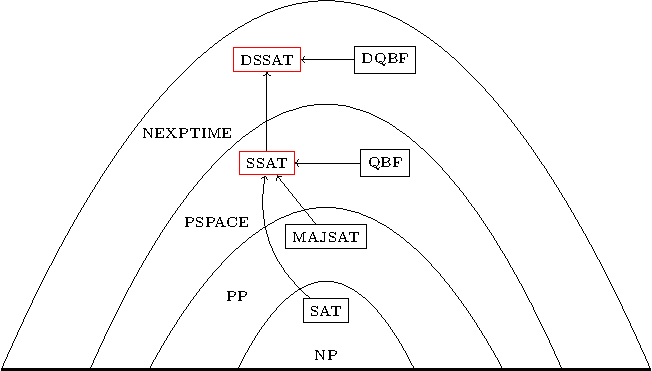
\includegraphics{fig/build/nutshell.pdf}
      \caption{The contributions of this dissertation in a nutshell}
      \label{fig:intro-nutshell}
\end{figure}

This dissertation aims at contributing to the aforementioned research needs.
Our achievements positioned in the hierarchy of various complexity classes beyond NP are visualized in~\cref{fig:intro-nutshell}.
In a nutshell, we investigate the application of SSAT to VLSI analysis,
leverage the advancements of SAT, MAJSAT, and QBF to design new decision procedures for SSAT,
and combine SSAT and DQBF to propose a new formulation, called DSSAT, for NEXPTIME problems with uncertainty.
In the following, we will explain each contribution in more detail.

First, we approach the analysis of probabilistic design by
formalizing the problem of \textit{probabilistic property evaluation}.
Different computational solutions are provided for the problem.
Particularly, random-exist and exist-random quantified SSAT formulas are exploited
to solve the average-case and worst-case analyses, respectively.
To the best of our knowledge,
this is the first attempt that analyzes VLSI systems with SSAT.
(In the following,
the terms ``analysis'' and ``evaluation'' are used interchangeably as general terms
referring to the process of determining qualitative or quantitative properties of a design.
We will formulate the problem of \textit{probabilistic property evaluation},
and refer to the term ``evaluation" as computing the satisfying probability of
certain properties of a probabilistic design.)

Second, in contrast to the previous DPLL-based algorithms,
we utilize modern techniques of SAT/QBF solving and model counting to improve SSAT solving.
Motivated by the new VLSI applications,
we focus on random-exist and exist-random quantified fragments of SSAT formulas.

The random-exist quantified SSAT formula is of the form $\Qf=\random{}X,\exists Y.\pf$,
which is the counterpart of the forall-exist QBF.
It has applications in Bayesian-network inference~\cite{Cooper1990,Bacchus2003}.
We propose an algorithm that uses modern SAT solvers~\cite{Een2003Solver,Een2003Incremental} as plug-in engines.
In addition to SAT solving,
we also incorporate weighted model counting,
which has been widely used in probabilistic inference~\cite{Sang2005BayesianInference,Chavira2008},
to tackle randomized quantifiers.
The randomized quantification in an SSAT formula can be approached with weighted model counting
by assigning the weight of a variable quantified by $\random{p}$ to be $p$.
The proposed algorithm uses an SAT solver and a model counter in a \textit{stand-alone} manner,
leaving the internal structures of these solvers intact.
Due to the stand-alone usage of these solvers,
the proposed algorithm may directly benefit from the advancement of the solvers without any modification.

The exist-random quantified SSAT formulas has the form $\Qf=\exists X,\random{}Y.\pf$,
which is also known as \textit{E-MAJSAT}~\cite{Littman1998}.
Computational problems, such as computing a maximum-a-posteriori (MAP) hypothesis or
a maximum-expected-utility (MEU) solution~\cite{Dechter1998} in Bayesian networks,
and searching an optimal plan for probabilistic conformant planning domains~\cite{Littman1998},
can be formulated with E-MAJSAT.
Inspired by the \textit{clause-selection}~\cite{Janota2015,Rabe2015} technique,
which is recently devised for QBF solving and becomes the state-of-the-art,
we propose a learning method based on the \textit{clause-containment principle} to solve E-MAJSAT.
To the best of our knowledge,
this is the first attempt to adopt QBF approaches for SSAT solving.

Moreover, the proposed algorithms solve an SSAT formula in a gradual manner
that converges from approximate bounds of the satisfying probability to the exact answer.
Therefore, they are able to provide useful information even if the exact answer is unavailable (e.g., due to limited computational resources).

Third, to provide a logical formalism for more complex problems with uncertainty,
we extend \textit{dependency QBF} (DQBF)~\cite{Balabanov2014,Scholl2018} to the stochastic domain
in view of the close relation between QBF and SSAT.
DQBF is a representative problem in the NEXPTIME-complete~\cite{Peterson2001} complexity class.
It equips QBF with Henkin quantifiers to describe multi-player games with partial information.
We formalize the problem of \textit{dependency SSAT} (DSSAT) as a generalization for SSAT.
We prove that DSSAT has the same NEXPTIME-complete complexity as DQBF,
and therefore it can succinctly encode decision problems with uncertainty in the NEXPTIME complexity class.
We demonstrate the potential applications of DSSAT to the synthesis of probabilistic and approximate design and the encoding of decentralized POMDP (Dec-POMDP)~\cite{Oliehoek2016} problems.
Our theoretical results would encourage the solver development.

Fourth, our implementation of the proposed SSAT algorithms
and formula instances used in the experiments are open-source,
which will help other researchers to understand the details of the approaches and
facilitate convenient empirical evaluation of different algorithms.

\section{An overview of the dissertation}
The structure of this dissertation is outlined as follows.
\begin{itemize}
      \item
            In~\cref{chap:related-work}, a brief survey of the literature is provided to highlight the advancements made in this dissertation.
      \item
            In~\cref{chap:background}, background knowledge required throughout the dissertation is discussed.
            Specific material for an individual chapter will be introduced when it is needed.
      \item
            In~\cref{chap:prob-design-eval}, a formal framework to evaluate properties of probabilistic design is proposed.
            Especially, random-exist and exist-random quantified SSAT formulas are exploited to solve the formulation.
            This chapter is based on our conference paper~\cite{LeeICCAD14ProbDesign} published at ICCAD\,'14 and journal paper~\cite{LeeTC18ProbDesign} published in IEEE Transactions on Computers.
      \item
            In~\cref{chap:random-exist-ssat}, modern SAT-solving and model-counting techniques are combined to solve random-exist quantified SSAT formulas.
            This chapter is based on our conference paper~\cite{LeeIJCAI17RESSAT} published at IJCAI\,'17.
      \item
            In~\cref{chap:exist-random-ssat}, a clause-learning technique inspired by \textit{clause selection}, a prevailing method recently invented for QBF, is devised to solve exist-random quantified SSAT formulas.
            This chapter is based on our conference paper~\cite{LeeIJCAI18ERSSAT} published at IJCAI\,'18.
      \item
            In~\cref{chap:dependency-ssat}, SSAT is lifted from the PSPACE-complete complexity class to the NEXPTIME-completeness.
            We show the applicability of the lifted formalism to the analysis of probabilistic design and decentralized POMDP.
            This chapter is based on our conference paper~\cite{LeeAAAI21DSSAT} published at AAAI\,'21.
      \item
            In~\cref{chap:conclusion-future-work}, we give concluding remarks and point out some potential directions for future investigation.
\end{itemize}